%%%%%%%%%%%%
%
% $Autor: Wings $
% $Datum: 2019-03-05 08:03:15Z $
% $Pfad: SDCard $
% $Version: 4250 $
% !TeX spellcheck = en_GB/de_DE
% !TeX encoding = utf8
% !TeX root = filename 
% !TeX TXS-program:bibliography = txs:///biber
%
%%%%%%%%%%%%

\chapter{Arduino - SD-Karten-Modul}

Ein \ac{spi}-Lesegerät ist eine Art Modul, das die Kommunikation zwischen einem Mikrocontroller und einer Speicherkarte, z. B. einer \ac{sd}- oder \ac{tf}-Karte, ermöglicht. Das Modul verwendet das \ac{spi}-Protokoll, um Daten zwischen den beiden Geräten zu übertragen. Das \ac{sd}/\ac{tf}-Card-Shield-Modul ist ein spezieller Typ von \ac{spi}-Leser, der für die Verwendung mit Mikrocontroller-Boards konzipiert ist. Es ermöglicht einen einfachen Zugriff auf die auf der Speicherkarte gespeicherten Daten und kann für eine Vielzahl von Anwendungen wie Datenprotokollierung, Dateispeicherung und Multimedia-Projekte verwendet werden. Das Shield wird über die \ac{spi}-Schnittstelle mit dem Mikrocontroller verbunden.

\begin{figure}[h]
    \begin{center}
        \includegraphics[width=12cm]{SDCard/SDCardSlot.png}
        \caption{SD/TF-Card-Shield-Modul}
        \label{fig:SD_Slot}
    \end{center}
\end{figure}

\section{Eigenschaften}

\begin{description}
    \item[Leichte und kostengünstige Erweiterung:] Der \ac{sd}-Karten Slot ermöglicht eine einfache und kostengünstige Erweiterung des Speicherplatzes für Ihr Arduino-Projekt mittels \ac{sd}-Karte.
    \item[Einfache Kommunikation:] Das Modul kommuniziert mit dem Mikrocontroller über das \ac{spi}-Protokoll, welches eine zuverlässige und schnelle Datenübertragung gewährleistet.
    \item[Unterstützung von Speicherkarten:] Es unterstützt sowohl Micro-SD-Karten (bis zu 2GB) als auch Micro-SDHC-Karten (bis zu 32GB), inklusive High-Speed-Karten.
    \item[Spannungsunterstützung:] Das Modul ist kompatibel mit einer Versorgungsspannung von 3,3-5V, was die Integration in verschiedene Projekte erleichtert.
\end{description}

\section{Technische Spezifikationen}

\begin{description}
    \item[Schnittstelle:] \ac{spi}
    \item[Unterstützte Karten:] Micro-SD-Karte (2GB), Micro-SDHC-Karte (bis zu 32GB)
    \item[Versorgungsspannung:] 3,3-5V
    \item[Kompatibilität:] Arduino und andere Mikrocontroller-Boards
\end{description}
\cite{AZ-Delivery:2021}



\section{Bibliothek \FILE{SD.h}}

Die SD.h Bibliothek ist eine essenzielle Bibliothek für Arduino-Entwickler, die es ermöglicht, \ac{sd}-Karten in ihren Projekten zu verwenden. Sie bietet eine einfache und effiziente Möglichkeit, Daten auf \ac{sd}-Karten zu speichern und zu lesen. Die Bibliothek unterstützt das FAT16 und FAT32 Dateisystem, was sie kompatibel mit den meisten \ac{sd}-Karten macht. Mit der SD.h Bibliothek können Dateien erstellt, gelöscht, umbenannt und bearbeitet werden. Zudem gibt es Funktionen zum Lesen und Schreiben von Daten in Dateien. Die Bibliothek ermöglicht das Erstellen und Löschen von Verzeichnissen (Ordnern) und unterstützt das Navigieren durch Verzeichnisse, was das Arbeiten mit komplexen Dateistrukturen erleichtert.

Die SD.h Bibliothek ist kompatibel mit den meisten Arduino-Boards, einschließlich Arduino Uno, Mega, Nano und anderen. Sie unterstützt sowohl Standard-\ac{sd}-Karten als auch microSD-Karten mit einem geeigneten Adapter. Die Integration der Bibliothek in Arduino-Sketches ist einfach und erfolgt durch leicht verständliche Methodenaufrufe. Die Arduino \ac{ide} enthält zudem Beispiele und umfangreiche Dokumentation, die den Einstieg in die Nutzung der SD.h Bibliothek erleichtern.


\section{Testen des SD-Karten Moduls}

Um das \ac{sd}-Karten Modul zu testen, haben wir ein Beispiel erstellt, das zeigt, wie man mit einem Arduino Daten auf einer \ac{sd}-Karte speichert und wieder ausliest. Basierend auf der Anleitung Funduino - Das \ac{sd}-Karten Modul haben wir den dortigen Beispielcode leicht angepasst \cite{AZ-Delivery:2021}. Zunächst wird die \ac{sd}-Karte initialisiert, um sicherzustellen, dass sie ordnungsgemäß funktioniert. Danach wird eine Testdatei erstellt, in die ein kurzer Text geschrieben wird. Anschließend wird der Inhalt dieser Datei ausgelesen und über den seriellen Monitor angezeigt.

\begin{code}[h]
    \pythonexternal[language=python]{../../Code/Arduino/SDCard/TestSDCard/TestSDCard.ino}
    \caption{Testprogramm SD-Karten-Modul} 
    \label{Code:Test_SD_Karten_Modul}
\end{code}

\begin{center}
    \includegraphics[width=10cm]{SDCard/SDCardTest}
    \captionof{figure}{Ausgabe SD-Kartentest Serieller Monitor}
    \label{fig:SD_Kartentest_Serieller_Monitor}	
\end{center}

\section{Entwicklerboard mit SD-Kartenleser}

Das \textit{Entwicklerboard mit SD-Kartenleser} \cite{AZDelivery.2024} ermöglicht eine einfache und kostengünstige Erweiterung des Arduino-Speicherplatzes durch einen integrierten Micro-SD-Kartenslot. Die Kommunikation mit dem Mikrocontroller erfolgt über das standardisierte SPI-Protokoll, was eine unkomplizierte Anbindung in bestehende Schaltungen erlaubt. Unterstützt werden sowohl Micro-SD-Karten mit einer Kapazität von bis zu 2 GB als auch Micro-SDHC-Karten mit bis zu 32 GB, einschließlich High-Speed-Karten. Der Betrieb des Moduls ist mit einer Versorgungsspannung von 3,3 - 5 V möglich, wodurch es direkt mit typischen Arduino-Boards kompatibel ist.

\bigskip

\begin{center}
    \includegraphics[width=7cm]{SDCard/SDCardSlot}
    \captionof{figure}{SD-Kartenleser}
    \label{fig: SD-Kartenleser}
\end{center}

\textit{* Für eine ausgiebige Aktorbeschreibung siehe:} Kapitel \ref{sec:SDKartenleser}. 


\section{SD-Karte}

Die eingesetzte microSD-Karte des Herstellers \glqq SanDisk\grqq{} entspricht dem gängigen Formfaktor microSD und basiert auf dem UHS-I-Busstandard, der vollständig abwärtskompatibel zum SPI-Modus (vgl. Abschnitt~\ref{sec:SPI}) ist und somit eine problemlose Anbindung an das SD-Modul des Arduino Nano 33 BLE Sense Lite ermöglicht. Für eine zuverlässige Nutzung mit der Arduino-\texttt{SD}-Library wird eine Kapazität von 32\,GB gewählt. Dadurch kann das weit verbreitete FAT32-Dateisystem genutzt werden, das in Mikrocontroller-Anwendungen als De-facto-Standard gilt und Dateien bis zu einer Größe von 4\,GB unterstützt. Die maximale Übertragungsgeschwindigkeit der Karte beträgt laut Hersteller bis zu 120\,MB/s, wobei in SPI-Anwendungen niedrigere Übertragungsraten üblich sind. \cite{WesternDigitalTechnologies.2022}

Intern arbeitet die SD-Karte mit nichtflüchtigem NAND-Flash-Speicher, der durch einen integrierten Controller verwaltet wird. Dieser übernimmt Aufgaben wie Wear-Leveling, Fehlerkorrektur (ECC) und Adressumsetzung (LBA), wodurch der Mikrocontroller die Speicherkarte wie ein gewöhnliches Blockgerät ansprechen kann. Diese interne Abstraktion ermöglicht einen einfachen Zugriff auf Dateien über Bibliotheken wie \texttt{SD.h} oder \texttt{SdFat}. \cite{Subero.2024}

Obwohl der UHS-I-Standard primär für Hochgeschwindigkeitsübertragungen über den nativen SD-Bus vorgesehen ist, unterstützt die Karte weiterhin den SPI-Modus im sogenannten „Backward Compatibility Mode“. Wird die Initialisierung über SPI durchgeführt, erkennt die SD-Karte dies automatisch und wechselt in den SPI-kompatiblen Betriebsmodus. Dadurch kann die Karte auch in ressourcenbeschränkten Systemen zuverlässig betrieben werden, ohne dass ein spezialisierter SD-Controller erforderlich ist.

Die Versorgungsspannung der SD-Karte beträgt 3{,}3\,V. Da viele Mikrocontroller (z.\,B. Arduino Uno) jedoch mit 5\,V-Logikpegeln arbeiten, ist eine Pegelanpassung erforderlich. Das verwendete SD-Kartenmodul enthält hierfür integrierte Spannungsregler und Pegelwandler, wodurch die Karte sowohl mit 3{,}3\,V- als auch mit 5\,V-Systemen kompatibel ist.


Die eingesetzte microSD-Karte des Herstellers \glqq SanDisk\grqq{} entspricht dem gängigen Formfaktor microSD und basiert auf dem UHS-I-Busstandard, der vollständig abwärtskompatibel zum SPI-Modus ist und somit eine problemlose Anbindung an das SD-Modul des Arduino Nano 33 BLE Sense Lite ermöglicht. Für eine zuverlässige Nutzung mit der Arduino SD-Library wird eine Kapazität von 32 GB gewählt, dadurch wird das FAT32-Dateisystem mit maximalem Speicherplatz genutzt. Die Übertragungsgeschwindigkeit beträgt bis zu 120 MB/s.
\cite{WesternDigitalTechnologies.2022} 
\href{../../../Documents/Datenblaetter/Datenbatt SD-Karte}{[Datenblatt.PDF]}


Die folgende Tabelle zeigt die Pinbelegung einer MicroSD-Karte sowohl im standardmäßigen SD-Modus als auch im SPI-Modus, der typischerweise bei Mikrocontroller-Projekten zum Einsatz kommt. Die physikalische Anordnung der Kontakte ist in Abbildung~\ref{fig:SDKarte} dargestellt. \cite{KingstonTechnology.2022}

\begin{table}[H]
    \centering
    \begin{tabular}{|c|c|c|p{8cm}|}
        \hline
        \textbf{Pin} & \textbf{SD-Modus} & \textbf{SPI-Modus} & \textbf{Funktion} \\
        \hline
        1 & DAT2         & –                 & Datenleitung 2 (nur im 4-Bit SD-Modus aktiv, im SPI-Modus ungenutzt) \\
        2 & CD / DAT3    & CS (Chip Select)  & Chip-Select-Signal zur Auswahl der Karte im SPI-Bus \\
        3 & CMD          & DI (Data In)      & Kommandoleitung, überträgt Befehle vom Host zur Karte (MOSI) \\
        4 & VDD          & VDD               & Versorgungsspannung (typisch 3{,}3\,V) \\
        5 & CLK          & SCLK              & Taktleitung für die Datenübertragung \\
        6 & VSS          & VSS               & Masseanschluss (Ground) \\
        7 & DAT0         & DO (Data Out)     & Datenleitung 0, überträgt Daten von der Karte zum Host (MISO) \\
        8 & DAT1         & –                 & Datenleitung 1 (nur im 4-Bit SD-Modus aktiv, im SPI-Modus ungenutzt) \\
        \hline
    \end{tabular}
    \caption{Pinbelegung einer MicroSD-Karte im SD- und SPI-Modus}
    \label{tab:microSD_Pinbelegung}
\end{table}
\vspace{1ex}

\begin{center}
	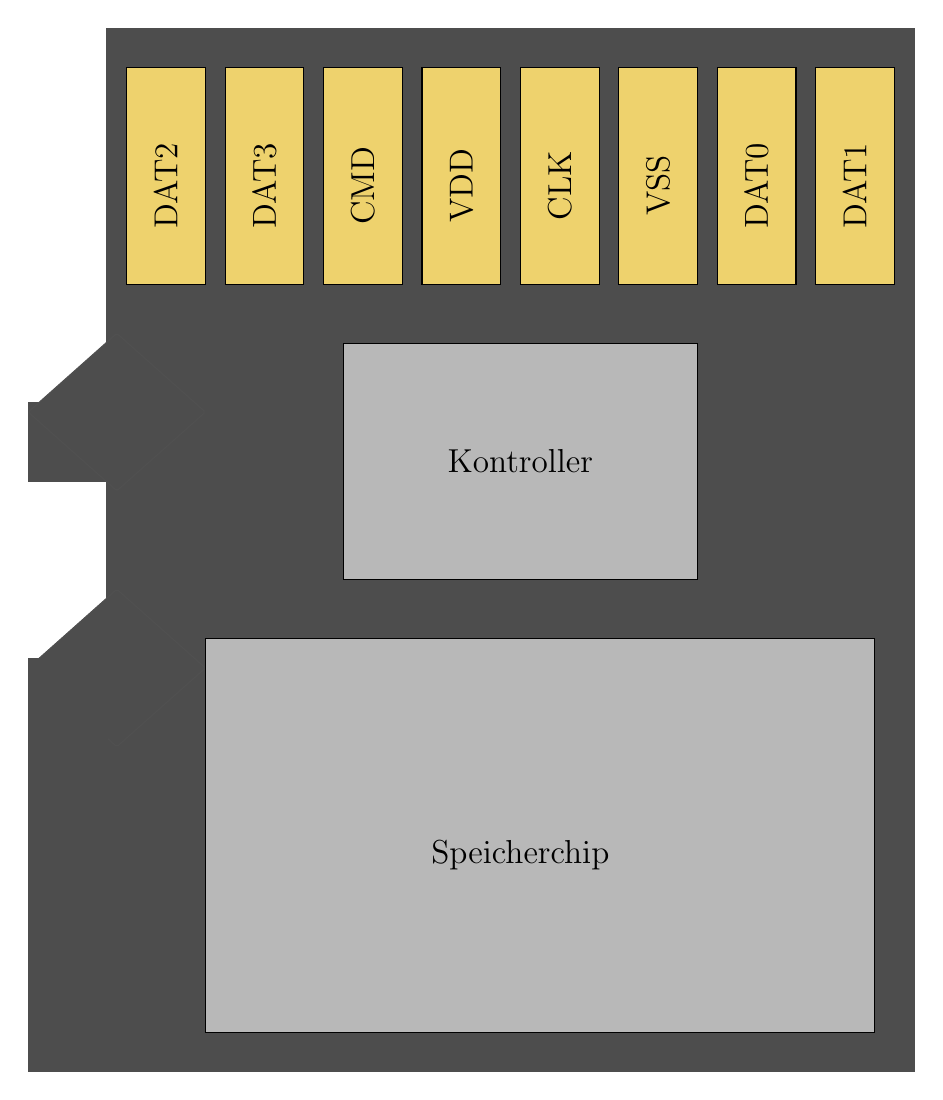
\begin{tikzpicture}		
    \draw [ color={rgb,255:red,77; green,77; blue,77} , fill={rgb,255:red,77; green,77; blue,77}] (16.25,17.5) rectangle (26.5,4.25);
    \draw [ color={rgb,255:red,80; green,80; blue,80} , fill={rgb,255:red,77; green,77; blue,77}, rounded corners = 0.6] (15.25,9.375) -- (16.375,8.375) -- (17.5,9.375) -- (16.375,10.375) -- cycle;
    \draw [ fill={rgb,255:red,238; green,210; blue,109} ] (16.5,17) rectangle (17.5,14.25);
    \node [font=\normalsize] at (17.5,16.25) {};
    \draw [ fill={rgb,255:red,238; green,210; blue,109} ] (17.75,17) rectangle (18.75,14.25);
    \draw [ color={rgb,255:red,77; green,77; blue,77} , fill={rgb,255:red,77; green,77; blue,77}] (15.25,9.5) rectangle (16.25,4.25);
    \draw [ color={rgb,255:red,77; green,77; blue,77} , fill={rgb,255:red,77; green,77; blue,77}] (15.25,12.75) rectangle (16.25,11.75);
    \draw [ color={rgb,255:red,80; green,80; blue,80} , fill={rgb,255:red,77; green,77; blue,77}, rounded corners = 0.6] (15.25,12.625) -- (16.375,11.625) -- (17.5,12.625) -- (16.375,13.625) -- cycle;
    \draw [ fill={rgb,255:red,238; green,210; blue,109} ] (19,17) rectangle (20,14.25);
    \draw [ fill={rgb,255:red,238; green,210; blue,109} ] (20.25,17) rectangle (21.25,14.25);
    \draw [ fill={rgb,255:red,238; green,210; blue,109} ] (21.5,17) rectangle (22.5,14.25);
    \draw [ fill={rgb,255:red,238; green,210; blue,109} ] (22.75,17) rectangle (23.75,14.25);
    \draw [ fill={rgb,255:red,238; green,210; blue,109} ] (24,17) rectangle (25,14.25);
    \node [font=\normalsize] at (22.75,15) {};
    \draw [ fill={rgb,255:red,238; green,210; blue,109} ] (25.25,17) rectangle (26.25,14.25);
    \draw [ fill={rgb,255:red,184; green,184; blue,184} ] (17.5,9.75) rectangle (26,4.75);
    \draw [ fill={rgb,255:red,184; green,184; blue,184} ] (19.25,13.5) rectangle (23.75,10.5);
    \node [font=\large] at (21.5,12) {Kontroller};
    \node [font=\large] at (21.5,7) {Speicherchip};
    \node [font=\large, rotate around={90:(0,0)}] at (17,15.5) {DAT2};
    \node [font=\large, rotate around={90:(0,0)}] at (18.25,15.5) {DAT3};
    \node [font=\large, rotate around={90:(0,0)}] at (19.5,15.5) {CMD};
    \node [font=\large, rotate around={90:(0,0)}] at (20.75,15.5) {VDD};
    \node [font=\large, rotate around={90:(0,0)}] at (22,15.5) {CLK};
    \node [font=\large, rotate around={90:(0,0)}] at (23.25,15.5) {VSS};
    \node [font=\large, rotate around={90:(0,0)}] at (24.5,15.5) {DAT0};
    \node [font=\large, rotate around={90:(0,0)}] at (25.75,15.5) {DAT1};
    
    
  \end{tikzpicture}
  \captionof{figure}{SD-Karte}
  \label{fig:SDKarte}
\end{center}

Im SPI-Modus sind nur vier Pins erforderlich:
\begin{itemize}
    \item \textbf{CS (Chip Select)} – Pin 2
    \item \textbf{MOSI (Data In)} – Pin 3
    \item \textbf{MISO (Data Out)} – Pin 7
    \item \textbf{SCK (Clock)} – Pin 5
\end{itemize}

Die übrigen Pins (DAT1, DAT2) bleiben im SPI-Betrieb ungenutzt. Die Versorgungsspannung liegt an Pin~4 (\textbf{VDD}), die Masseleitung an Pin~6 (\textbf{VSS}).


\begin{itemize}
    \item \textbf{CS (Chip Select) – Pin 2:}  
    Dient zur Auswahl des SD-Kartenmoduls im SPI-Bus. Wird vom Mikrocontroller auf \texttt{LOW} gezogen, um die Kommunikation mit der Karte zu aktivieren. Nur ein Gerät im SPI-Bus darf gleichzeitig ausgewählt sein.
    
    \item \textbf{MOSI (Master Out Slave In) – Pin 3:}  
    Überträgt Daten und Befehle vom Mikrocontroller (Master) zur SD-Karte (Slave). Dieser Pin wird im SD-Modus als \texttt{CMD} bezeichnet.
    
    \item \textbf{MISO (Master In Slave Out) – Pin 7:}  
    Überträgt Daten von der SD-Karte zum Mikrocontroller. Dieser Pin entspricht im SD-Modus der Leitung \texttt{DAT0}.
    
    \item \textbf{SCK (Serial Clock) – Pin 5:}  
    Liefert den Takt, mit dem die Datenübertragung im SPI-Protokoll synchronisiert wird. Der Takt wird vom Master (also vom Mikrocontroller) erzeugt.
\end{itemize}


\section{Entwicklerboard mit SD-Kartenleser}

Das \textit{Entwicklerboard mit SD-Kartenleser} \cite{AZDelivery.2024} ermöglicht eine Erweiterung des Arduino-Speicherplatzes durch einen integrierten Micro-SD-Kartenslot. Die Kommunikation mit dem Mikrocontroller erfolgt über das standardisierte SPI-Protokoll. Unterstützt werden sowohl Micro-SD-Karten mit einer Kapazität von bis zu 2 GB als auch Micro-SDHC-Karten mit bis zu 32 GB, einschließlich High-Speed-Karten. Der Betrieb des Moduls ist mit einer Versorgungsspannung von 3,3 - 5 V möglich.

\bigskip

\begin{center}
    \includegraphics[width=7cm]{SDCard/SDCardSlot}
    \captionof{figure}{SD-Kartenleser}
    \label{fig: SD-Kartenleser}
\end{center}

\textit{* Für eine ausgiebige Aktorbeschreibung siehe:} Kapitel \ref{sec:SDKartenleser}. 


\section{SD-Karte}

Die eingesetzte microSD-Karte des Herstellers „SanDisk“ entspricht dem gängigen Formfaktor microSD und basiert auf dem UHS-I-Busstandard, der vollständig abwärtskompatibel zum SPI-Modus (vgl. Abschnitt~\ref{sec:SPI}) ist und somit eine problemlose Anbindung an das SD-Modul des Arduino Nano 33 BLE Sense Lite ermöglicht. Für eine zuverlässige Nutzung mit der Arduino-\texttt{SD}-Library wird eine Kapazität von 32\,GB gewählt. Dadurch kann das weit verbreitete FAT32-Dateisystem genutzt werden, das in Mikrocontroller-Anwendungen als De-facto-Standard gilt und Dateien bis zu einer Größe von 4\,GB unterstützt. Die maximale Übertragungsgeschwindigkeit der Karte beträgt laut Hersteller bis zu 120\,MB/s, wobei in SPI-Anwendungen niedrigere Übertragungsraten üblich sind. \cite{WesternDigitalTechnologies.2022}

Intern arbeitet die SD-Karte mit nichtflüchtigem NAND-Flash-Speicher, der durch einen integrierten Controller verwaltet wird. Dieser übernimmt Aufgaben wie Wear-Leveling, Fehlerkorrektur (ECC) und Adressumsetzung (LBA), wodurch der Mikrocontroller die Speicherkarte wie ein gewöhnliches Blockgerät ansprechen kann. Diese interne Abstraktion ermöglicht einen einfachen Zugriff auf Dateien über Bibliotheken wie \texttt{SD.h} oder \texttt{SdFat}. \cite{Subero.2024}

Obwohl der UHS-I-Standard primär für Hochgeschwindigkeitsübertragungen über den nativen SD-Bus vorgesehen ist, unterstützt die Karte weiterhin den SPI-Modus im sogenannten „Backward Compatibility Mode“. Wird die Initialisierung über SPI durchgeführt, erkennt die SD-Karte dies automatisch und wechselt in den SPI-kompatiblen Betriebsmodus. Dadurch kann die Karte auch in ressourcenbeschränkten Systemen zuverlässig betrieben werden, ohne dass ein spezialisierter SD-Controller erforderlich ist.

Die Versorgungsspannung der SD-Karte beträgt 3{,}3\,V. Da viele Mikrocontroller (z.\,B. Arduino Uno) jedoch mit 5\,V-Logikpegeln arbeiten, ist eine Pegelanpassung erforderlich. Das verwendete SD-Kartenmodul enthält hierfür integrierte Spannungsregler und Pegelwandler, wodurch die Karte sowohl mit 3{,}3\,V- als auch mit 5\,V-Systemen kompatibel ist.


Die eingesetzte microSD-Karte des Herstellers „SanDisk“ entspricht dem gängigen Formfaktor microSD und basiert auf dem UHS-I-Busstandard, der vollständig abwärtskompatibel zum SPI-Modus ist und somit eine problemlose Anbindung an das SD-Modul des Arduino Nano 33 BLE Sense Lite ermöglicht. Für eine zuverlässige Nutzung mit der Arduino SD-Library wird eine Kapazität von 32 GB gewählt, dadurch wird das FAT32-Dateisystem mit maximalem Speicherplatz genutzt. Die Übertragungsgeschwindigkeit beträgt bis zu 120 MB/s.
\cite{WesternDigitalTechnologies.2022} 
\href{../../../Documents/Datenblaetter/Datenbatt SD-Karte}{[Datenblatt.PDF]}


Die folgende Tabelle zeigt die Pinbelegung einer MicroSD-Karte sowohl im standardmäßigen SD-Modus als auch im SPI-Modus, der typischerweise bei Mikrocontroller-Projekten zum Einsatz kommt. Die physikalische Anordnung der Kontakte ist in Abbildung~\ref{fig:SDKarte} dargestellt. \cite{KingstonTechnology.2022}

\begin{center}
    \begin{tabular}{|c|c|c|p{8cm}|}
        \hline
        \textbf{Pin} & \textbf{SD-Modus} & \textbf{SPI-Modus} & \textbf{Funktion} \\
        \hline
        1 & DAT2         & –                 & Datenleitung 2 (nur im 4-Bit SD-Modus aktiv, im SPI-Modus ungenutzt) \\
        2 & CD / DAT3    & CS (Chip Select)  & Chip-Select-Signal zur Auswahl der Karte im SPI-Bus \\
        3 & CMD          & DI (Data In)      & Kommandoleitung, überträgt Befehle vom Host zur Karte (MOSI) \\
        4 & VDD          & VDD               & Versorgungsspannung (typisch 3{,}3\,V) \\
        5 & CLK          & SCLK              & Taktleitung für die Datenübertragung \\
        6 & VSS          & VSS               & Masseanschluss (Ground) \\
        7 & DAT0         & DO (Data Out)     & Datenleitung 0, überträgt Daten von der Karte zum Host (MISO) \\
        8 & DAT1         & –                 & Datenleitung 1 (nur im 4-Bit SD-Modus aktiv, im SPI-Modus ungenutzt) \\
        \hline
    \end{tabular}
    \captionof{table}{Pinbelegung einer MicroSD-Karte im SD- und SPI-Modus}
    \label{tab:microSD_Pinbelegung}
\end{center}

\bigskip

\begin{center}
	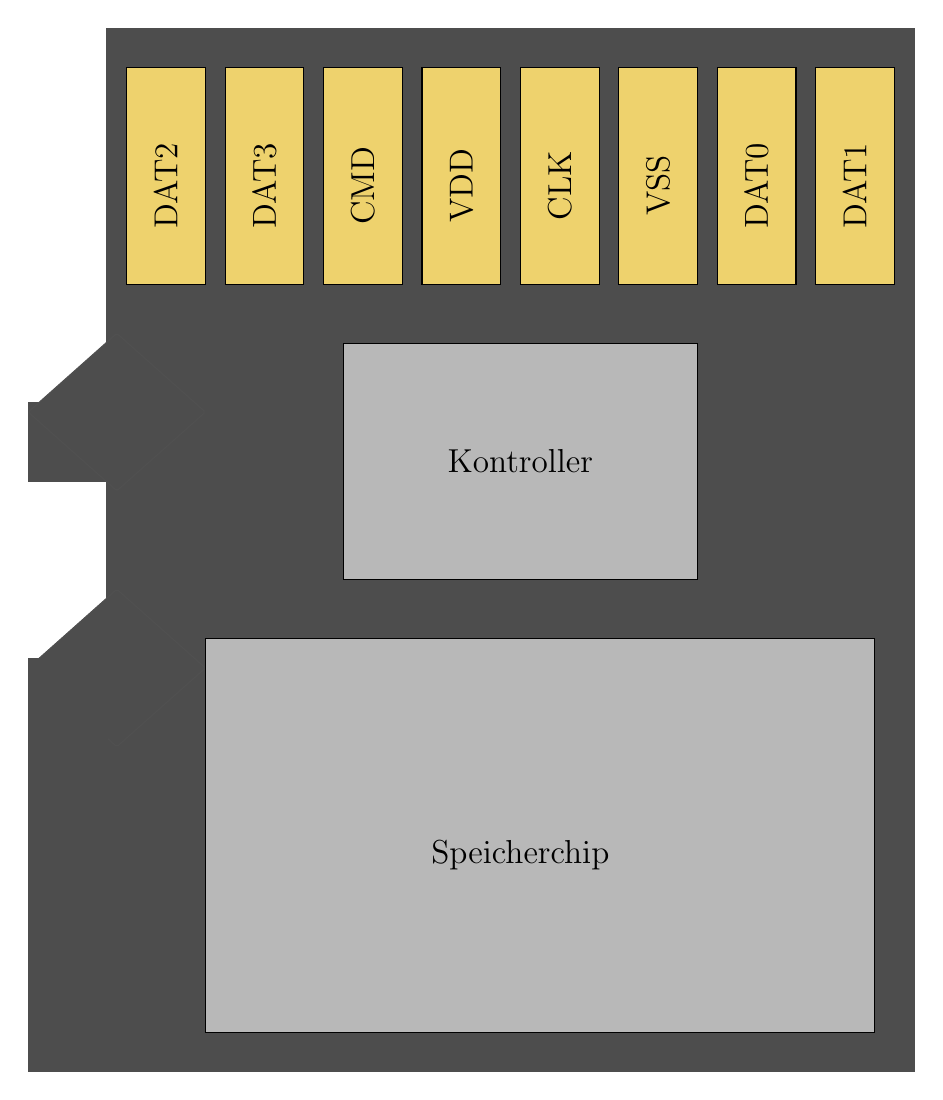
\begin{tikzpicture}		
    \draw [ color={rgb,255:red,77; green,77; blue,77} , fill={rgb,255:red,77; green,77; blue,77}] (16.25,17.5) rectangle (26.5,4.25);
    \draw [ color={rgb,255:red,80; green,80; blue,80} , fill={rgb,255:red,77; green,77; blue,77}, rounded corners = 0.6] (15.25,9.375) -- (16.375,8.375) -- (17.5,9.375) -- (16.375,10.375) -- cycle;
    \draw [ fill={rgb,255:red,238; green,210; blue,109} ] (16.5,17) rectangle (17.5,14.25);
    \node [font=\normalsize] at (17.5,16.25) {};
    \draw [ fill={rgb,255:red,238; green,210; blue,109} ] (17.75,17) rectangle (18.75,14.25);
    \draw [ color={rgb,255:red,77; green,77; blue,77} , fill={rgb,255:red,77; green,77; blue,77}] (15.25,9.5) rectangle (16.25,4.25);
    \draw [ color={rgb,255:red,77; green,77; blue,77} , fill={rgb,255:red,77; green,77; blue,77}] (15.25,12.75) rectangle (16.25,11.75);
    \draw [ color={rgb,255:red,80; green,80; blue,80} , fill={rgb,255:red,77; green,77; blue,77}, rounded corners = 0.6] (15.25,12.625) -- (16.375,11.625) -- (17.5,12.625) -- (16.375,13.625) -- cycle;
    \draw [ fill={rgb,255:red,238; green,210; blue,109} ] (19,17) rectangle (20,14.25);
    \draw [ fill={rgb,255:red,238; green,210; blue,109} ] (20.25,17) rectangle (21.25,14.25);
    \draw [ fill={rgb,255:red,238; green,210; blue,109} ] (21.5,17) rectangle (22.5,14.25);
    \draw [ fill={rgb,255:red,238; green,210; blue,109} ] (22.75,17) rectangle (23.75,14.25);
    \draw [ fill={rgb,255:red,238; green,210; blue,109} ] (24,17) rectangle (25,14.25);
    \node [font=\normalsize] at (22.75,15) {};
    \draw [ fill={rgb,255:red,238; green,210; blue,109} ] (25.25,17) rectangle (26.25,14.25);
    \draw [ fill={rgb,255:red,184; green,184; blue,184} ] (17.5,9.75) rectangle (26,4.75);
    \draw [ fill={rgb,255:red,184; green,184; blue,184} ] (19.25,13.5) rectangle (23.75,10.5);
    \node [font=\large] at (21.5,12) {Kontroller};
    \node [font=\large] at (21.5,7) {Speicherchip};
    \node [font=\large, rotate around={90:(0,0)}] at (17,15.5) {DAT2};
    \node [font=\large, rotate around={90:(0,0)}] at (18.25,15.5) {DAT3};
    \node [font=\large, rotate around={90:(0,0)}] at (19.5,15.5) {CMD};
    \node [font=\large, rotate around={90:(0,0)}] at (20.75,15.5) {VDD};
    \node [font=\large, rotate around={90:(0,0)}] at (22,15.5) {CLK};
    \node [font=\large, rotate around={90:(0,0)}] at (23.25,15.5) {VSS};
    \node [font=\large, rotate around={90:(0,0)}] at (24.5,15.5) {DAT0};
    \node [font=\large, rotate around={90:(0,0)}] at (25.75,15.5) {DAT1};
    
    
  \end{tikzpicture}
  \captionof{figure}{SD-Karte}
  \label{fig:SDKarte}
\end{center}

Im SPI-Modus sind nur vier Pins erforderlich:

\begin{itemize}
    \item \textbf{CS (Chip Select)} – Pin 2
    \item \textbf{MOSI (Data In)} – Pin 3
    \item \textbf{MISO (Data Out)} – Pin 7
    \item \textbf{SCK (Clock)} – Pin 5
\end{itemize}

Die übrigen Pins (DAT1, DAT2) bleiben im SPI-Betrieb ungenutzt. Die Versorgungsspannung liegt an Pin~4 (\textbf{VDD}), die Masseleitung an Pin~6 (\textbf{VSS}).


\begin{itemize}
    \item \textbf{CS (Chip Select) – Pin 2:}  
    Dient zur Auswahl des SD-Kartenmoduls im SPI-Bus. Wird vom Mikrocontroller auf \texttt{LOW} gezogen, um die Kommunikation mit der Karte zu aktivieren. Nur ein Gerät im SPI-Bus darf gleichzeitig ausgewählt sein.
    
    \item \textbf{MOSI (Master Out Slave In) – Pin 3:}  
    Überträgt Daten und Befehle vom Mikrocontroller (Master) zur SD-Karte (Slave). Dieser Pin wird im SD-Modus als \texttt{CMD} bezeichnet.
    
    \item \textbf{MISO (Master In Slave Out) – Pin 7:}  
    Überträgt Daten von der SD-Karte zum Mikrocontroller. Dieser Pin entspricht im SD-Modus der Leitung \texttt{DAT0}.
    
    \item \textbf{SCK (Serial Clock) – Pin 5:}  
    Liefert den Takt, mit dem die Datenübertragung im SPI-Protokoll synchronisiert wird. Der Takt wird vom Master (also vom Mikrocontroller) erzeugt.
\end{itemize}


\chapter{SD-Karten-Modul}\label{SD-Karten-Modul}


Ein \ac{spi}-Lesegerät ist ein Modul, das die Kommunikation zwischen einem Mikrocontroller und einer Speicherkarte, z. B. einer \ac{sd}- oder \ac{tf}-Karte, ermöglicht. Das Modul verwendet das \ac{spi}-Protokoll, um Daten zwischen den beiden Geräten zu übertragen. Das \ac{sd}/\ac{tf}-Card-Shield-Modul ist ein spezieller Typ von \ac{spi}-Leser, der für die Verwendung mit Mikrocontroller-Boards konzipiert ist. Es ermöglicht den Zugriff auf gespeicherte Daten auf der SD-Karte und kann für eine Vielzahl von Anwendungen wie Datenprotokollierung, Dateispeicherung und Multimedia-Projekte verwendet werden. Das Shield wird über die \ac{spi}-Schnittstelle mit dem Mikrocontroller verbunden(Abbildung~\ref{fig:SD_Slot}).\cite{AZDelivery2025}

Ein \ac{spi}-Lesegerät ist eine Art Modul, das die Kommunikation zwischen einem Mikrocontroller und einer Speicherkarte, z. B. einer \ac{sd}- oder \ac{tf}-Karte, ermöglicht. Das Modul verwendet das \ac{spi}-Protokoll, um Daten zwischen den beiden Geräten zu übertragen. Das \ac{sd}/\ac{tf}-Card-Shield-Modul ist ein spezieller Typ von \ac{spi}-Leser, der für die Verwendung mit Mikrocontroller-Boards konzipiert ist. Es ermöglicht einen einfachen Zugriff auf die auf der Speicherkarte gespeicherten Daten und kann für eine Vielzahl von Anwendungen wie Datenprotokollierung, Dateispeicherung und Multimedia-Projekte verwendet werden. Das Shield wird über die \ac{spi}-Schnittstelle mit dem Mikrocontroller verbunden(Abbilung~\ref{fig:SD_Slot}).\cite{AZDelivery2025}

\begin{center}
	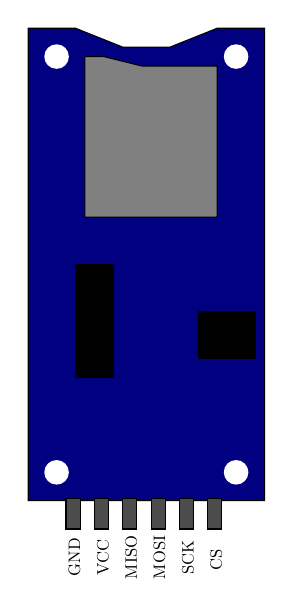
\begin{tikzpicture}[scale=1.2]
		% Vergrößerte Platine
		\filldraw [fill=blue!50!black](0,0) -- (0,5)--(0.5,5)--(1,4.8)--(1.5,4.8)--(2,5)--(2.5,5)--(2.5,0)--cycle;
		\filldraw [fill=black!50](0.6,3) -- (0.6,4.7)--(0.8,4.7)--(1.2,4.6)--(2,4.6)--(2,3)--cycle;
		\filldraw [fill=black!120](1.8,1.5) -- (1.8,2)-- (2.4,2)--(2.4,1.5)--cycle;
		\filldraw [fill=black!100](0.5,1.3) -- (0.5,2.5)-- (0.9,2.5)--(0.9,1.3)--cycle;
		% Bohrlöcher
		\foreach \x/\y in {0.3/0.3, 0.3/4.7, 2.2/4.7, 2.2/0.3} {
			\fill [white] (\x,\y) circle (0.13);
		}
		\foreach \i/\name in {
			0/GND,
			1/VCC,
			2/MISO,
			3/MOSI,
			4/SCK,
			5/CS
		} { 
			\pgfmathsetmacro\y{0.1 -\i * 0.3}
			\filldraw[fill=black!70] ( 0.5-\y,-0.3) rectangle +(0.15, 0.32);
			\node[anchor=center, text=black, rotate=90] at (0.59-\y, -0.6) {\scalebox{0.6}{\name}};
		}
	\end{tikzpicture}
	\captionof{figure}{SD-Karten-Modul nach \cite{funduinoSD2025} }
	\label{fig:SD_Slot}
\end{center}

\section{Eigenschaften}

\begin{description}
	\item[Leichte und kostengünstige Erweiterung:] Der \ac{sd}-Karten-Slot ermöglicht eine einfache und kostengünstige Erweiterung des Speicherplatzes für Ihr Arduino-Projekt mittels \ac{sd}-Karte.
	\item[Einfache Kommunikation:] Das Modul kommuniziert mit dem Mikrocontroller über das \ac{spi}-Protokoll, welches eine zuverlässige und schnelle Datenübertragung gewährleistet.
	\item[Unterstützung von Speicherkarten:] Es unterstützt sowohl Micro-SD-Karten (bis zu 2~~GB) als auch Micro-SDHC-Karten (bis zu 32~GB), inklusive High-Speed-Karten.
	\item[Spannungsunterstützung:] Das Modul ist kompatibel mit einer Versorgungsspannung von 3,3-5V, was die Integration in verschiedene Projekte erleichtert.\cite{AZDelivery2025}
\end{description}

\section{Technische Spezifikationen}

Dies ist in der folgenden Tabelle \ref{tab:Technische Spezifikationen} dargestellt. Für das Projekt Schlüsselkasten ist insbesondere die 3.3~V Kompatibilität entscheidend.

\begin{center}
	\captionof{table}{Technische Spezifikationen: SD-Karten-Modul  	\cite{funduinoSD2025}}\label{tab:Technische Spezifikationen}
	\begin{tabular}{|l|l|}
		
		\hline
		Schnittstelle&\ac{spi} \\
		\hline
		Unterstützte Karten& Micro-SD-Karte (2\,GB), Micro-SDHC-Karte (bis zu 32GB) \\
		\hline
		Versorgungsspannung& 3,3-5~V \\
		\hline
		Kompatibilität&  Arduino und andere Mikrocontroller-Boards  \\
		\hline
	\end{tabular}
\end{center}


\section{Bibliothek \FILE{SD.h}}


Die \PYTHON{SD.h} Bibliothek ist eine Bibliothek für Arduino-Entwickler, die es ermöglicht, \ac{sd}-Karten in ihren Projekten zu verwenden. Sie bietet eine einfache und effiziente Methode, Daten auf \ac{sd}-Karten zu speichern und zu lesen. Die Bibliothek unterstützt das FAT16 und FAT32 Dateisystem, was sie kompatibel mit den meisten \ac{sd}-Karten macht. Mit der \PYTHON{SD.h} Bibliothek können Dateien erstellt, gelöscht, umbenannt und bearbeitet werden. Zudem gibt es Funktionen zum Lesen und Schreiben von Daten in Dateien. Die Bibliothek ermöglicht das Erstellen und Löschen von Verzeichnissen (Ordnern) und unterstützt das Navigieren durch Verzeichnisse, was das Arbeiten mit komplexen Dateistrukturen erleichtert.



\section{Testen des SD-Karten-Moduls}

Um das \ac{sd}-Karten Modul zu testen, haben wir ein Beispiel erstellt(Listing~\ref{Code:Test_SD_Karten_Modul}), das zeigt, wie man mit einem Arduino Daten auf einer \ac{sd}-Karte speichert und wieder ausliest. Basierend auf der Anleitung Funduino - Das \ac{sd}-Karten Modul haben wir den dortigen Beispielcode leicht angepasst \cite{AZDelivery2025}. Zunächst wird die \ac{sd}-Karte initialisiert, um sicherzustellen, dass sie ordnungsgemäß funktioniert. Danach wird eine Testdatei erstellt, in die ein kurzer Text geschrieben wird. Anschließend wird der Inhalt dieser Datei ausgelesen und über den seriellen Monitor angezeigt (Abbilung~\ref{fig:SD_Kartentest_Serieller_Monitor}).

\subsection{Anschluss am Tiny Machine Learning Shield}
Die Pins GND und 3.3~V werden später an die Grove Schnittstelle angeschlossen, da diese für den RFID-Sensor verwendet werden. Für den ersten Test werden die Pins wie in Abbildung \ref{fig:pins_shield_SD} beschrieben angeschlossen. Bei den Pins handelt es sich um digitale Pins, diese sind aus dem Schaltplans des Tiny Machine Learning Shields \ref{fig:TML_Cam} zu entnehmen. 


\begin{center}
	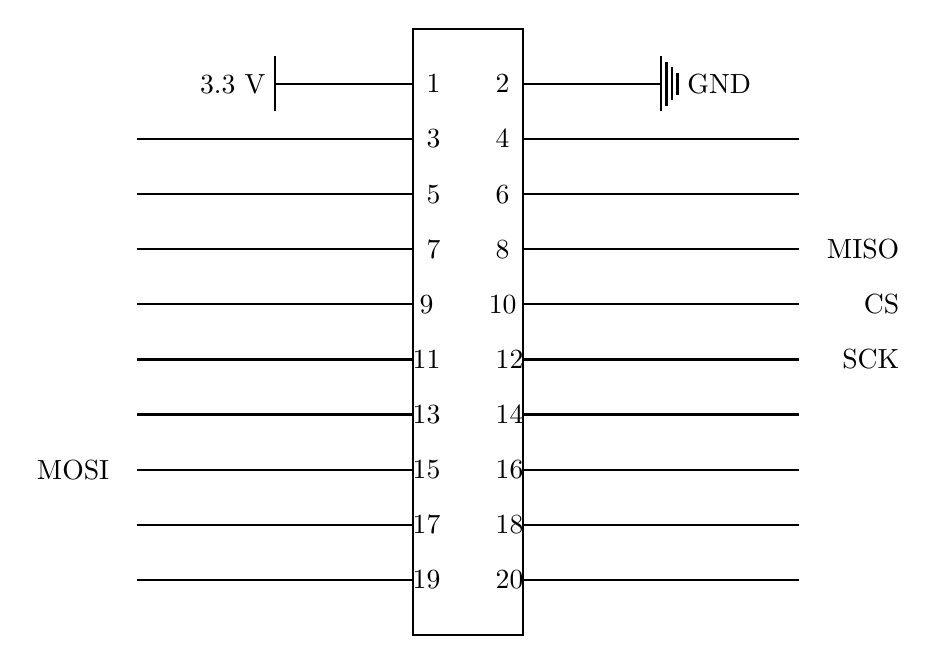
\begin{tikzpicture}[scale=0.7]
		% Rechteck
		\draw[thick] (5, 0) rectangle (7, 11);
		
		% Linien mit Beschriftung und Innenbeschriftung
		\foreach \y/\leftlabel/\rightlabel/\leftdesc/\rightdesc in {
			1/19/20//,
			2/17/18//,
			3/15/16/MOSI/,
			4/13/14//,
			5/11/12//SCK,
			6/9/10//CS,
			7/7/8//MISO,
			8/5/6//,
			9/3/4//,
			10/1/2/ /
		} {
			% Sonderfall: 3 V (Linie 10)
			\ifnum\y=10
			\draw[thick] (2.5,\y) -- (5,\y); % linke Linie gekürzt
			\node[anchor=center] at (6,\y) {\leftlabel\quad\quad\rightlabel}; % Rechteck-Beschriftung
			\node[anchor=west] at (2.5,\y) {\leftdesc}; % Beschreibung links
			\node[anchor=east] at (9.5,\y) {\rightdesc}; % Beschreibung rechts
			\draw[thick] (2.5,9.5) -- (2.5,10.5); % senkrechte 3V Linie
			\node[left] at (2.5, 10) {3.3~V};
			\draw[thick] (9.5,9.5) -- (9.5,10.5); % GND Linie
			\draw[thick] (9.6,9.6) -- (9.6,10.4);
			\draw[thick] (9.7,9.7) -- (9.7,10.3);
			\draw[thick] (9.8,9.8) -- (9.8,10.2);
			\node[right] at (9.8, 10) {GND};
			\draw[thick] (7,\y) -- (9.5,\y); % rechte Linie ganz
			% Sonderfall: GND (Linie 9)
			\else\ifnum\y=9
			% Sonderfall GND hier behandeln (falls benötigt)
			\draw[thick] (0,\y) -- (5,\y); % linke Linie
			\draw[thick] (7,\y) -- (12,\y); % rechte Linie
			\node[anchor=center] at (6,\y) {\leftlabel\quad\quad\rightlabel}; % Zahlen im Rechteck
			\node[anchor=west] at (-1,\y) {\leftdesc}; % Beschreibung links
			\node[anchor=east] at (13,\y) {\rightdesc}; % Beschreibung rechts
			% Alle anderen Pins
			\else
			\draw[thick] (0,\y) -- (5,\y); % linke Linie
			\draw[thick] (7,\y) -- (12,\y); % rechte Linie
			% Zahlen im Rechteck (weiter auseinander)
			\node[anchor=center] at (6,\y) {\leftlabel\quad\quad\rightlabel}; % Zahlen im Rechteck
			\node[anchor=west] at (-2,\y) {\leftdesc}; % Beschreibung links
			\node[anchor=east] at (14,\y) {\rightdesc}; % Beschreibung rechts
			\fi\fi
		}
	\end{tikzpicture}
	\captionof{figure}{Pins des Shields nach  \cite{ArduinoShield:2021} und \ref{TinyMachineLearningShieldPins}\label{fig:pins_shield_SD}}
\end{center}

\subsection{Testprogramm des SD-Karten Moduls}

{
	\captionof{code}{Testprogramm für das SD-Karten-Modul} 
	\label{Code:Test_SD_Karten_Modul}
	\ArduinoExternal{}{../../Code/Arduino/SDCard/TestSDCard/TestSDCard.ino}
	
}

\begin{center}
	\includegraphics[width=10cm]{SDCard/SDCardTest}
	\captionof{figure}{Ausgabe SD-Kartentest Serieller Monitor [eigene Darstellung]}
	\label{fig:SD_Kartentest_Serieller_Monitor}	
\end{center}

\chapter{SD-Karten-Modul}
\label{ch:SDKartenModul}

Das \ac{sd}-Karten-Modul dient als Schnittstelle zwischen einem Mikrocontroller und einer Micro\ac{sd}-Karte. Es ermöglicht das Speichern und Auslesen von Messdaten. \cite{veeramanikandasamy_microcontroller_2016}

%---------------------------------------------------------------------------------------------------------------------------%

\section{Allgemeine Beschreibung}

Eine \acs{sd}-Karte ist ein nichtflüchtiges Speichermedium, welches entwickelt wurde, um vor allem eine wiederbeschreibbare Speicherlösung zu schaffen \cite {vaishnavi_arduino_2021}. Es handelt sich um ein \ac{spi} basiertes Speichermodul, welches eine zuverlässige und schnelle Übertragung von großen Datenmengen ermöglicht \cite{veeramanikandasamy_microcontroller_2016}. Seltener wird auch ein SD-Bus, auch SDIO genannt, zur Kommunikation genutzt \cite{veeramanikandasamy_microcontroller_2016}.
\\
\acs{sd}-Karten-Module ermöglichen Mikrocontrollersystemen also den Zugriff auf dieses nichtflüchtige Speichermedium. Es wird verwendet, um Daten wie Messwerte, Log-Dateien oder Konfigurationsinformationen lokal zu speichern. Das ist vor allem bei Systemen relevant, bei denen keine dauerhafte Verbindung zu einem Netzwerk besteht. Ein typisches Anwendungsbeispiel aufgrund der unabhängigen und stromsparenden Messung ist die Datenprotokollierung, zum Beispiel zur Langzeitüberwachung von Solarenergieanlagen \cite{hadi_standalone_2018}. Darüber hinaus können \acs{sd}-Karten-Module zur Maschinenüberwachung in Industrieanlagen verwendet werden, indem sie Daten von Sensoren auffassen in Textdateien speichern \cite{veeramanikandasamy_microcontroller_2016}. Häufig sind die Module mit einer Real Time Clock verknüpft, um eine Zeitstempelung vorzusehen. Dies ist auch der Fall in der Datenprotokollierung von Umweltdaten, welche dann später zusammen mit dem Zeitstempel ausgewertet werden können \cite{vaishnavi_arduino_2021}. Dadurch sind solche Module ebenfalls für die Bildung und Lehre, Forschung und Entwicklung, als auch für die Prototypenentwicklung und Hobby-Projekte geeignet \cite{roboter-bausatzde_micro_2025}.
\\
Die Module erlauben die grundlegenden Dateioperationen wie Erstellen, Lesen, Schreiben und Löschen. Die erzeugten Dateien lassen sich ohne zusätzliche Treiber oder Tools weiterverarbeiten und können analysiert werden. Dadurch sind sie sowohl für die temporäre, als auch für die permanente Speicherung von Daten geeignet.
Je nach Modul sind verschiedene \acs{sd}-Karten-Formate und unterschiedliche Bauarten verfügbar, sodass viele Möglichkeiten zur Einbindung in Mikrocontrollersystemen bestehen. Zudem unterscheiden sie sich hinsichtlich der unterstützten Dateisystemen, der Schnittstelle und der Logikpegel.\\

\acs{sd}-Karten lassen sich bezüglich ihrer Kapazitäten und der Dateisysteme in vier Klassen einteilen:
\begin{itemize}
    \item \textbf{SDSC:}
    Standard Capacity, bis zu 2GB, formatiert mit \acs{fat}12 oder \acs{fat}16
    \item \textbf{SDHC:}
    High Capacity, 4GB bis 32GB, formatiert mit \acs{fat}32
    \item \textbf{SDXC:}
    Extended Capacity, 64GB bis 2TB, formatiert mit ex\acs{fat}
    \item \textbf{SDUC:}
    Ultra Capacity, bis zu 128TB, formatiert mit ex\acs{fat}
\end{itemize}

Die maximale Dateisystemgröße bei \acs{fat}12 beträgt dabei lediglich 16MB, weshalb es als veraltet betrachtet wird. Außerdem ist das ex\acs{fat}-Dateisystem von Microsoft patentiert und dementsprechend lizenzpflichtig. Es wird in Mikrocontroller-Umgebungen nur eingeschränkt genutzt und beispielsweise von der \texttt{SD.h} Bibliothek nicht unterstützt. Das Acronym \acs{fat} steht dabei für File Allocation Table und bezeichnet ein einfaches, tabellenbasiertes Dateisystem, bei dem die Speicherbelegung in einer zentralen Zuordnungstabelle verwaltet wird. \cite{baun_operating_2023}

%---------------------------------------------------------------------------------------------------------------------------%

\section{Micro SD Card Reader}

Das \ac{sd}-Karten-Modul, welches in der Abbildung \ref{fig:SDCard_Pinout} gezeigt wird, unterstützt sowohl Micro\ac{sd}-, als auch Micro \ac{sdhc}-Karten mit einer Kapazität von bis zu 32GB. Die Kommunikation mit dem Mikrocontroller erfolgt dabei über den \acs{spi}-Bus mit den folgenden vier Leitungen: \ac{cs}, \ac{mosi}, \ac{miso} und \ac{sck} \cite{veeramanikandasamy_microcontroller_2016}. Das Modul ist so ausgelegt, dass es mit Mikrocontrollern arbeiten kann, welche 5 V-Logik nutzen. Dafür enthält es einen integrierten AMS1117-3.3 Spannungsregler, welcher die Betriebsspannung für die \acs{sd}-Karte auf 3,3 V absenkt. Zusätzlich sind Pegelwandler für die \acs{spi}-Signale auf dem \acs{sd}-Karten-Modul vorhanden.  \cite{az-delivery_vertriebs_gmbh_sd-karten-modul_2015} \cite{roboter-bausatzde_micro_2025}\\

\begin{figure}
    \centering
    \resizebox{0.45\textwidth}{!}{%
        \begin{tikzpicture}
            \tikzstyle{every node}=[font=\LARGE]
            \draw [ color={rgb,255:red,254; green,254; blue,254} , fill={rgb,255:red,55; green,85; blue,144}, rounded corners = 15.6] (7.25,17.75) rectangle (12,10.5);
            \draw [ color={rgb,255:red,55; green,85; blue,144} , fill={rgb,255:red,168; green,168; blue,168}, rounded corners = 3.0] (8.25,17.25) rectangle (11,15.25);
            \draw [ color={rgb,255:red,55; green,85; blue,144} , fill={rgb,255:red,254; green,254; blue,254}, line width=2pt ] (7.75,11) circle (0.25cm);
            \draw [ color={rgb,255:red,55; green,85; blue,144} , fill={rgb,255:red,254; green,254; blue,254}, line width=2pt ] (11.5,11) circle (0.25cm);
            \draw [ color={rgb,255:red,55; green,85; blue,144} , fill={rgb,255:red,254; green,254; blue,254}, line width=2pt ] (11.5,17.25) circle (0.25cm);
            \draw [ color={rgb,255:red,55; green,85; blue,144} , fill={rgb,255:red,254; green,254; blue,254}, line width=2pt ] (7.75,17.25) circle (0.25cm);
            \draw [ color={rgb,255:red,255; green,255; blue,255} , fill={rgb,255:red,69; green,69; blue,69}, rounded corners = 3.0] (8.25,13.5) rectangle (9,12.5);
            \draw [ color={rgb,255:red,255; green,255; blue,255} , fill={rgb,255:red,69; green,69; blue,69}, rounded corners = 3.0] (10.5,13.5) rectangle (11.25,13);
            \draw [ color={rgb,255:red,255; green,255; blue,255} , fill={rgb,255:red,69; green,69; blue,69}, rounded corners = 3.0] (8,11.5) rectangle (11.25,11);
            \draw [ color={rgb,255:red,255; green,255; blue,255} , fill={rgb,255:red,168; green,168; blue,168}, rounded corners = 3.0] (8.25,11.25) rectangle (8.5,9.25);
            \node [font=\LARGE] at (9.5,9.75) {};
            \node [font=\LARGE] at (9.5,9.75) {};
            \draw [ color={rgb,255:red,255; green,255; blue,255} , fill={rgb,255:red,168; green,168; blue,168}, rounded corners = 3.0] (8.75,11.25) rectangle (9,9.25);
            \draw [ color={rgb,255:red,255; green,255; blue,255} , fill={rgb,255:red,168; green,168; blue,168}, rounded corners = 3.0] (9.25,11.25) rectangle (9.5,9.25);
            \draw [ color={rgb,255:red,255; green,255; blue,255} , fill={rgb,255:red,168; green,168; blue,168}, rounded corners = 3.0] (9.75,11.25) rectangle (10,9.25);
            \draw [ color={rgb,255:red,255; green,255; blue,255} , fill={rgb,255:red,168; green,168; blue,168}, rounded corners = 3.0] (10.25,11.25) rectangle (10.5,9.25);
            \draw [ color={rgb,255:red,255; green,255; blue,255} , fill={rgb,255:red,168; green,168; blue,168}, rounded corners = 3.0] (10.75,11.25) rectangle (11,9.25);
            \draw [line width=1pt, short] (8.25,9) -- (8.25,8.5);
            \draw [line width=1pt, short] (8.25,8.5) -- (7,8.5);
            \draw [line width=1pt, short] (8.75,9) -- (8.75,8);
            \draw [line width=1pt, short] (8.75,8) -- (7.75,8);
            \draw [line width=1pt, short] (9.25,9) -- (9.25,7.5);
            \draw [line width=1pt, short] (9.25,7.5) -- (8.5,7.5);
            \draw [line width=1pt, short] (11,9) -- (11,8.5);
            \draw [line width=1pt, short] (11,8.5) -- (12.25,8.5);
            \draw [line width=1pt, short] (10.5,9) -- (10.5,8);
            \draw [line width=1pt, short] (10.5,8) -- (11.5,8);
            \draw [line width=1pt, short] (10,9) -- (10,7.5);
            \draw [line width=1pt, short] (10,7.5) -- (10.75,7.5);
            \node [font=\large] at (6.25,8.5) {GND};
            \node [font=\large] at (7,8) {VCC};
            \node [font=\large] at (7.75,7.5) {MISO};
            \node [font=\large] at (12.75,8.5) {CS};
            \node [font=\large] at (12.25,8) {SCK};
            \node [font=\large] at (11.5,7.5) {MOSI};
            \draw [ color={rgb,255:red,255; green,255; blue,255} , fill={rgb,255:red,55; green,85; blue,144}, line width=1pt ] (7.75,14.75) rectangle (8.25,13.75);
            \draw [ color={rgb,255:red,255; green,255; blue,255} , fill={rgb,255:red,55; green,85; blue,144}, line width=1pt ] (8.5,14.75) rectangle (9,13.75);
            \node [font=\LARGE, color={rgb,255:red,255; green,255; blue,255}] at (8.75,13.75) {};
            \draw [ color={rgb,255:red,255; green,255; blue,255} , fill={rgb,255:red,55; green,85; blue,144}, line width=1pt ] (7.5,12.75) rectangle (8,11.75);
            \draw [ color={rgb,255:red,255; green,255; blue,255} , fill={rgb,255:red,55; green,85; blue,144}, line width=1pt ] (11.25,12.75) rectangle (11.75,11.75);
            \node [font=\LARGE, color={rgb,255:red,255; green,255; blue,255}] at (12,11.75) {};
            \node [font=\LARGE, color={rgb,255:red,255; green,255; blue,255}] at (12.5,11.25) {};
            \draw [ color={rgb,255:red,255; green,255; blue,255} , fill={rgb,255:red,55; green,85; blue,144}, line width=1pt ] (10.5,12.75) rectangle (11,11.75);
            \draw [ color={rgb,255:red,255; green,255; blue,255} , fill={rgb,255:red,55; green,85; blue,144}, line width=1pt ] (9.75,12.75) rectangle (10.25,11.75);
            \node [font=\LARGE, color={rgb,255:red,255; green,255; blue,255}] at (9.25,13.75) {};
            \node [font=\LARGE, color={rgb,255:red,255; green,255; blue,255}] at (9.25,13.75) {};
            \draw [ color={rgb,255:red,255; green,255; blue,255} , fill={rgb,255:red,55; green,85; blue,144}, line width=1pt ] (10.5,14.75) rectangle (11,13.75);
            \draw [ color={rgb,255:red,255; green,255; blue,255} , fill={rgb,255:red,55; green,85; blue,144}, line width=1pt ] (11.25,14.75) rectangle (11.75,13.75);
            \draw [ color={rgb,255:red,55; green,85; blue,144} , fill={rgb,255:red,226; green,182; blue,106}, line width=0.2pt ] (7.75,14.5) rectangle (8.25,14);
            \draw [ color={rgb,255:red,55; green,85; blue,144} , fill={rgb,255:red,226; green,182; blue,106}, line width=0.2pt ] (8.5,14.5) rectangle (9,14);
            \draw [ color={rgb,255:red,55; green,85; blue,144} , fill={rgb,255:red,226; green,182; blue,106}, line width=0.2pt ] (7.5,12.5) rectangle (8,12);
            \draw [ color={rgb,255:red,55; green,85; blue,144} , fill={rgb,255:red,226; green,182; blue,106}, line width=0.2pt ] (11.25,12.5) rectangle (11.75,12);
            \draw [ color={rgb,255:red,55; green,85; blue,144} , fill={rgb,255:red,41; green,41; blue,41}, line width=0.2pt ] (9.75,12.5) rectangle (10.25,12);
            \draw [ color={rgb,255:red,55; green,85; blue,144} , fill={rgb,255:red,41; green,41; blue,41}, line width=0.2pt ] (10.5,12.5) rectangle (11,12);
            \draw [ color={rgb,255:red,55; green,85; blue,144} , fill={rgb,255:red,41; green,41; blue,41}, line width=0.2pt ] (10.5,14.5) rectangle (11,14);
            \draw [ color={rgb,255:red,55; green,85; blue,144} , fill={rgb,255:red,41; green,41; blue,41}, line width=0.2pt ] (11.25,14.5) rectangle (11.75,14);
            \draw [ color={rgb,255:red,199; green,199; blue,199} , fill={rgb,255:red,199; green,199; blue,199}, line width=2pt ] (10,15.25) rectangle (10,15);
            \node [font=\LARGE, color={rgb,255:red,199; green,199; blue,199}] at (10.5,14.75) {};
            \node [font=\LARGE, color={rgb,255:red,199; green,199; blue,199}] at (10.5,14.75) {};
            \node [font=\LARGE, color={rgb,255:red,199; green,199; blue,199}] at (10.5,14.75) {};
            \draw [ color={rgb,255:red,199; green,199; blue,199} , fill={rgb,255:red,199; green,199; blue,199}, line width=2pt ] (10.25,15.25) rectangle (10.25,15);
            \draw [ color={rgb,255:red,199; green,199; blue,199} , fill={rgb,255:red,199; green,199; blue,199}, line width=2pt ] (9.75,15.25) rectangle (9.75,15);
            \draw [ color={rgb,255:red,199; green,199; blue,199} , fill={rgb,255:red,199; green,199; blue,199}, line width=2pt ] (10.5,15.25) rectangle (10.5,15);
            \draw [ color={rgb,255:red,199; green,199; blue,199} , fill={rgb,255:red,199; green,199; blue,199}, line width=2pt ] (10.75,15.25) rectangle (10.75,15);
            \draw [ color={rgb,255:red,199; green,199; blue,199} , fill={rgb,255:red,199; green,199; blue,199}, line width=2pt ] (9.5,15.25) rectangle (9.5,15);
            \draw [ color={rgb,255:red,199; green,199; blue,199} , fill={rgb,255:red,199; green,199; blue,199}, line width=2pt ] (9.25,15.25) rectangle (9.25,15);
            \draw [ color={rgb,255:red,199; green,199; blue,199} , fill={rgb,255:red,199; green,199; blue,199}, line width=2pt ] (9,15.25) rectangle (9,15);
            \draw [ color={rgb,255:red,199; green,199; blue,199} , fill={rgb,255:red,199; green,199; blue,199}, line width=2pt , rotate around={90:(8.25, 13.125)}] (8.25,13.25) rectangle (8.25,13);
            \draw [ color={rgb,255:red,199; green,199; blue,199} , fill={rgb,255:red,199; green,199; blue,199}, line width=2pt , rotate around={90:(8.25, 12.875)}] (8.25,13) rectangle (8.25,12.75);
            \draw [ color={rgb,255:red,199; green,199; blue,199} , fill={rgb,255:red,199; green,199; blue,199}, line width=2pt , rotate around={90:(8.25, 13.375)}] (8.25,13.5) rectangle (8.25,13.25);
            \draw [ color={rgb,255:red,199; green,199; blue,199} , fill={rgb,255:red,199; green,199; blue,199}, line width=0.2pt , rotate around={-90:(9, 13.125)}] (9.25,13.25) rectangle (8.75,13);
            \draw [ fill={rgb,255:red,0; green,0; blue,0} , line width=2pt ] (8.25,9.5) rectangle (8.5,8.75);
            \draw [ color={rgb,255:red,255; green,0; blue,0} , fill={rgb,255:red,255; green,0; blue,0}, line width=2pt ] (8.75,9.5) rectangle (9,8.75);
            \draw [ color={rgb,255:red,4; green,0; blue,255} , fill={rgb,255:red,4; green,0; blue,255}, line width=2pt ] (9.25,9.5) rectangle (9.5,8.75);
            \draw [ color={rgb,255:red,4; green,255; blue,0} , fill={rgb,255:red,4; green,255; blue,0}, line width=2pt ] (9.75,9.5) rectangle (10,8.75);
            \draw [ color={rgb,255:red,251; green,255; blue,0} , fill={rgb,255:red,251; green,255; blue,0}, line width=2pt ] (10.25,9.5) rectangle (10.5,8.75);
            \draw [ color={rgb,255:red,217; green,217; blue,217} , fill={rgb,255:red,245; green,245; blue,245}, line width=2pt ] (10.75,9.5) rectangle (11,8.75);
        \end{tikzpicture}
    }%
    \caption{Pinout des SD-Karten-Moduls}
    \label{fig:SDCard_Pinout}
\end{figure}

Vom Modul werden Speicherkarten mit \acs{fat}16- oder \acs{fat}32-Dateisystemen unterstützt. SDXC- oder SDUC-Karten ab 64GB mit exFAT-Formatierung müssen vor Verwendung auf \acs{fat}32 umformatiert werden. Dafür können Formatierungstools aus dem Internet genutzt werden.\\

%---------------------------------------------------------------------------------------------------------------------------%

\section{Eigenschaften}

Die wichtigsten technischen Eigenschaften des Moduls sind nach den Datenblättern \cite{roboter-bausatzde_micro_2025} \cite{az-delivery_vertriebs_gmbh_sd-karten-modul_2015} folgende:

\begin{itemize}
    \item Micro\acs{sd}-Karten-Modul zur Speichererweiterung über \ac{spi}-Schnittstelle. 
    Erlaubt das Schreiben und Lesen von Daten auf Micro\ac{sd}- und Micro\ac{sdhc}-Karten.
    \item Unterstützt Micro\ac{sd}-Karten bis 2 GB sowie Micro\ac{sdhc}-Karten bis 32 GB. 
    \item Eingangsspannung: 3,3 V bis 5,5 V.
    \item Interner AMS1117-3.3 Spannungsregler auf 3,3 V vorhanden.
    Schutz der \ac{sd}-Karte vor Überspannung durch automatische Spannungsanpassung.
    \item Anschlussbelegung: \acs{gnd}, \acs{vcc}, \acs{miso}, \acs{mosi}, \acs{sck}, \acs{cs}. 
    \item Kompatibel mit 3,3 V- und 5 V-Logiksystemen. 
    Geeignet für viele Mikrocontroller-Plattformen wie Arduino Nano, Arduino Uno, Mega, ESP32 und STM32.
    \item Integrierte Pegelwandler vorhanden. 
    Erhöht die Betriebssicherheit bei Verwendung von 5 V-Logiksystemen.
    \item Abmessungen des Moduls: ca. 41 mm x 24 mm.
    \item Gewicht: ca. 5 g.
\end{itemize}

\medskip

\begin{figure}
    \centering
    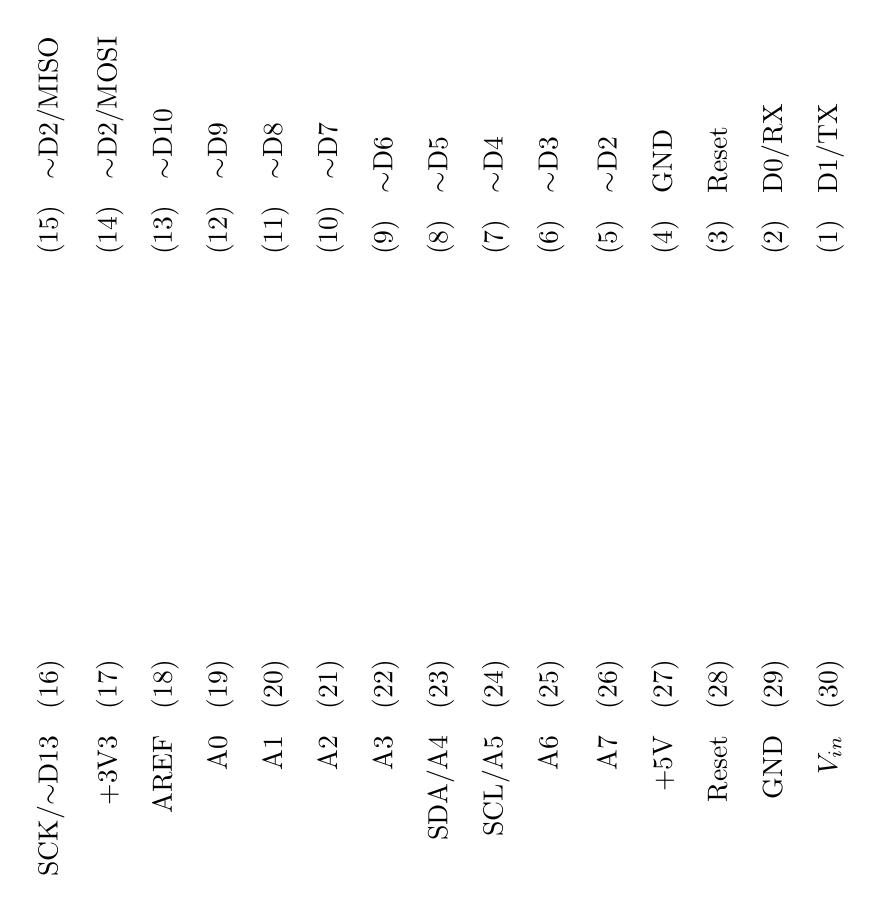
\begin{tikzpicture}
        
        \ArduinoNanoBLESenseRev
        
        \node[rotate=90,right] (Pin1) at (11.2,4.9) {(1) \; D1/TX};
        \node[rotate=90,right] (Pin2) at (10.5,4.9) {(2) \; D0/RX};
        \node[rotate=90,right] (Pin3) at (9.8,4.9) {(3) \; Reset};
        \node[rotate=90,right] (Pin4) at (9.1,4.9) {(4) \; GND};
        \node[rotate=90,right] (Pin5) at (8.4,4.9) {(5) \; $\sim$D2};
        \node[rotate=90,right] (Pin6) at (7.65,4.9) {(6) \; $\sim$D3};
        \node[rotate=90,right] (Pin7) at (6.95,4.9) {(7) \; $\sim$D4};
        \node[rotate=90,right] (Pin8) at (6.25,4.9) {(8) \; $\sim$D5};
        \node[rotate=90,right] (Pin9) at (5.55,4.9) {(9) \; $\sim$D6};
        \node[rotate=90,right] (Pin10) at (4.85,4.9) {(10) \; $\sim$D7};
        \node[rotate=90,right] (Pin11) at (4.15,4.9) {(11) \; $\sim$D8};
        \node[rotate=90,right] (Pin12) at (3.45,4.9) {(12) \; $\sim$D9};
        \node[rotate=90,right] (Pin13) at (2.75,4.9) {(13) \; $\sim$D10};
        \node[rotate=90,right] (Pin14) at (2.05,4.9) {(14) \; $\sim$D2/MOSI};
        \node[rotate=90,right] (Pin15) at (1.3,4.9) {(15) \; $\sim$D2/MISO};
        
        
        \node[rotate=90,left] (Pin30) at (11.2,-0.0) { $V_{in}$ \; (30)};
        \node[rotate=90,left] (Pin1) at (10.5,-0.0) {GND \; (29)};
        \node[rotate=90,left] (Pin2) at (9.8,-0.0) {Reset \; (28)};
        \node[rotate=90,left] (Pin3) at (9.1,-0.0) {+5V \; (27)};
        \node[rotate=90,left] (Pin4) at (8.4,-0.0) {A7 \; (26)};
        \node[rotate=90,left] (Pin5) at (7.65,-0.0) {A6 \; (25)};
        \node[rotate=90,left] (Pin6) at (6.95,-0.0) {SCL/A5 \; (24)};
        \node[rotate=90,left] (Pin7) at (6.25,-0.0) {SDA/A4 \; (23)};
        \node[rotate=90,left] (Pin8) at (5.55,-0.0) {A3 \; (22)};
        \node[rotate=90,left] (Pin9) at (4.85,-0.0) {A2 \; (21)};
        \node[rotate=90,left] (Pin10) at (4.15,-0.0) {A1 \; (20)};
        \node[rotate=90,left] (Pin11) at (3.45,-0.0) {A0 \; (19)};
        \node[rotate=90,left] (Pin12) at (2.75,-0.0) {AREF \; (18)};
        \node[rotate=90,left] (Pin13) at (2.05,-0.0) {+3V3 \; (17)};
        \node[rotate=90,left] (Pin14) at (1.3,-0.0) {SCK/$\sim$D13 \; (16)};
        
    \end{tikzpicture}
    \caption{Pinout des Arduino Nano 33 BLE Sense Lite}
    \label{fig:Nano_Lite_Pinout}
\end{figure}

\begin{figure}
    \begin{center}
        \includegraphics[width=8cm]{../../Images/SDCard/SketchPinBoard.png}
        \caption{Schaltplan \ac{sd}-Karten-Modul und Arduino Nano 33 BLE Sense Lite}
        \label{fig:SD_Karten_Schaltplan}
    \end{center}
\end{figure}

Für die Spannungsversorgung wird der 3,3 V- oder 5 V-Ausgang des Arduino genutzt (17, 27), der über den integrierten Spannungsregler des Moduls auf 3,3~V angepasst wird (rote Leitung). 
Die Masseleitungen (29) beider Systeme werden verbunden, um ein gemeinsames Bezugspotential zu gewährleisten (schwarze Leitung).

Die Signalleitungen sind wie folgt zugeordnet:
\begin{itemize}
    \item \textbf{Grüne Leitung:} Verbindet den Pin D11 bzw. D2/MOSI (14) des Arduino mit dem \acs{mosi}-Pin des \acs{sd}-Moduls.
    \item \textbf{Blaue Leitung:} Verbindet den Pin D12 bzw. D2/MISO (15) des Arduino mit dem \acs{miso}-Pin des \acs{sd}-Moduls.
    \item \textbf{Gelbe Leitung:} Verbindet den Pin D13 bzw. SCK/~D13 (16) des Arduino mit dem \acs{sck}-Pin des \acs{sd}-Moduls.
    \item \textbf{Weiße Leitung:} Verbindet den digitalen Pin D10 (13) des Arduino mit dem \acs{cs}-Pin des \acs{sd}-Moduls.
\end{itemize}

%---------------------------------------------------------------------------------------------------------------------------%

\section{Bibliothek \FILE{SD.h}}

\subsection{Beschreibung}

Zur Ansteuerung des \ac{sd}-Karten-Moduls wird die \texttt{SD.h} Bibliothek verwendet.
Mit dieser können Dateien auf der Speicherkarte erstellt, gelesen, beschrieben, gelöscht und umbenannt werden. Darüber hinaus ermöglicht sie das Anlegen und Verwalten von Verzeichnissen, was den Umgang mit komplexeren Dateistrukturen erleichtert.

Die \texttt{SD.h} Bibliothek ist kompatibel mit einer Vielzahl von Arduino-Boards, darunter Arduino Nano, Mega, Uno sowie weitere Modelle.
Die Integration der Bibliothek in Arduino-Sketches erfolgt über leicht verständliche Funktionsaufrufe.
Zusätzlich bietet die Arduino IDE Beispiele und eine umfangreiche Dokumentation, die den Einstieg in die Nutzung der Bibliothek unterstützt.

\subsection{Installation}

Die \texttt{SD.h} Bibliothek ist standardmäßig in der Arduino IDE enthalten und muss daher nicht separat installiert werden.
Sie kann direkt über die integrierte Bibliotheksverwaltung eingebunden und verwendet werden. Dafür müssen zunächst folgende Header eingegeben werden:

\begin{verbatim}
    #include <SPI.h>
    #include <SD.h>
\end{verbatim}

Die Bibliothek verwendet \PYTHON{File}-Objekte für Dateioperationen. Verarbeitet werden insbesondere die Datentypen \PYTHON{byte}, \PYTHON{char} und \PYTHON{String}, die für den Zugriff auf Dateien und Verzeichnisse genutzt werden.
Die maximale Dateigröße und die Anzahl der Dateien richten sich nach der Kapazität der verwendeten Micro\acs{sd}- oder Micro\acs{sdhc}-Karte.
Beispielsketche zur Anwendung der Bibliothek finden sich in der Arduino IDE, wie in Abbildung \ref{fig:SDCard_BeispielSketches} gezeigt, unter \menu{Datei}\textrightarrow \menu{Beispiele}\textrightarrow \menu{SD}.  \cite{arduino_sd_2024}

\begin{figure}
    \begin{center}
        \includegraphics[width=12cm]{../../Images/SDCard/ExampleSketch.png}
        \caption{Beispielsketches der \FILE{SD.h}}
        \label{fig:SDCard_BeispielSketches}
    \end{center}
\end{figure}

\subsection{Funktionen innerhalb der Bibliothek}

Die \FILE{SD.h} Bibliothek stellt Funktionen bereit, die den Zugriff auf Dateien und Verzeichnisse der SD-Karte ermöglichen. 
Wichtige Funktionen sind nach \cite{arduino_sd_2024} folgende:

\begin{itemize}
    \item \PYTHON{SD.begin(chipSelectPin)}: Initialisiert die SD-Karte über den angegebenen Chip-Select-Pin und bereitet sie für den Zugriff vor.
    \item \PYTHON{SD.exists(filepath)}: Prüft, ob eine Datei oder ein Verzeichnis mit dem angegebenen Pfad auf der SD-Karte existiert.
    \item \PYTHON{SD.open(filepath, mode)}: Öffnet eine Datei auf der \acs{sd}-Karte im angegebenen Modus (\PYTHON{FILE\_READ} oder \PYTHON{FILE\_WRITE}) und gibt ein \PYTHON{File}-Objekt zurück.
    \item \PYTHON{SD.remove(filepath)}: Löscht die Datei mit dem angegebenen Pfad von der \acs{sd}-Karte.
    \item \PYTHON{SD.mkdir(filepath)}: Erstellt ein neues Verzeichnis auf der \acs{sd}-Karte mit dem angegebenen Pfad.  
    \item \PYTHON{SD.rmdir(filepath)}: Entfernt ein leeres Verzeichnis mit dem angegebenen Pfad von der \acs{sd}-Karte.
    \\
    \item \PYTHON{file.available()}: Gibt die Anzahl der Bytes zurück, die aus der geöffneten Datei gelesen werden können.
    \item \PYTHON{file.read()}: Liest das nächste Byte aus der geöffneten Datei und gibt es als \PYTHON{int} zurück.
    \item \PYTHON{file.peek()}: Gibt das nächste Byte zurück, ohne den Lesezeiger in der Datei zu verschieben.
    \item \PYTHON{file.write(data)}: Schreibt ein Byte oder einen Datenpuffer in die geöffnete Datei.
    \item \PYTHON{file.print(data)}: Schreibt Daten in die Datei als Text ohne abschließenden Zeilenumbruch.
    \item \PYTHON{file.println(data)}: Schreibt Daten in die Datei als Text, gefolgt von einem Zeilenumbruch.
    \item \PYTHON{file.flush()}: Erzwingt das Schreiben aller gepufferten Daten auf die \acs{sd}-Karte.
    \item \PYTHON{file.close()}: Schließt die geöffnete Datei und gibt belegte Ressourcen frei. 
\end{itemize}

%---------------------------------------------------------------------------------------------------------------------------%

\section{Testen der Funktionen}
\subsection{Beschreibung}

In der Beispielanwendung soll die Nutzung des SD-Karten-Moduls in Verbindung mit dem Mikrocontroller getestet werden. Dabei wird zunächst überprüft, ob eine eingelegte Speicherkarte korrekt erkannt und angesprochen werden kann. Anschließend wird versucht eine neue Textdatei auf der Karte anzulegen oder eine vorhandene zu öffnen. In dieser Datei wird dann ein kurzer Text geschrieben, um die Funktionalität des Moduls zu testen. 
\\
Nach dem Schreiben wird die Datei wieder geschlossen und danach erneut geöffnet. Diesmal soll der zuvor gespeicherte Inhalt ausgelesen werden. Dadurch können alle zentralen Funktionen getestet werden.

\subsection{Umsetzung mit der \FILE{SD.h} Bibliothek}

Mithilfe des Codes \ref{lst:SDCardExample} kann die Funktionalität des SD-Karten-Moduls getestet werden. Zu Beginn wird die \acs{sd}-Karte mithilfe von \PYTHON{SD.begin(chipSelectPin)} initialisiert. Dabei wird der CS-Pin übergeben. Wenn die Karte erkannt wurde, kann das Dateisystem geladen und auf Dateien zugegriffen werden. Die Funktion gibt in diesem Fall \PYTHON{true} zurück. Falls das fehlschlägt, so wird die Ausführung abgebrochen und entsprechend \PYTHON{false} zurückgegeben.\\

Danach wird mithilfe von \PYTHON{SD.open("test.txt", FILE\_WRITE)} eine Datei mit dem Namen \PYTHON{test.txt} geöffnet. Existiert diese zu dem Zeitpunkt noch nicht, so wird sie neu angelegt. Diese Funktion liefert ein \PYTHON{File}-Objekt zurück. Dieses kann mit \PYTHON{if(file)} geprüft werden.\\

Bei erfolgreichem Öffnen wird über \PYTHON{file.println("Testeintrag")} ein einfacher Text in die Datei geschrieben. Danach kann mit \PYTHON{file.close()} sichergestellt werden, dass alle Daten auf die Karte übertragen und die Datei abgeschlossen wird.\\

Zur Überprüfung der Schreibfunktion wird dieselbe Datei erneut geöffnet, diesmal im Lesenmodus mit \PYTHON{SD.open("test.txt", FILE\_READ)}. Danach können die Inhalte mit \PYTHON{file.available()} und \PYTHON{file.read()} ausgelesen und über die serielle Schnittstelle angezeigt werden. Danach wird die Datei wieder mit \PYTHON{file.close()} geschlossen.

{
    \captionof{code}{Initialisierung und Testen des \acs{sd}-Karten-Moduls} \label{lst:SDCardExample}
    \ArduinoExternal{}{../../Code/Arduino/SDCard/Example/Example.ino}
}

%\begin{code}
%	\ArduinoExternal{linerange={1-64}, firstnumber=1}{../../Code/Arduino/SDCard/SDCardExample/SDCardExample.ino}
%	\label{Code:SDCardExample}
%\end{code}
%
%\begin{code}
%	\ArduinoExternal{linerange={65-88}, firstnumber=65}{../../Code/Arduino/SDCard/SDCardExample/SDCardExample.ino}
%	\caption{Initialisierung und Testen des SD-Karten-Moduls} 
%\end{code}

%---------------------------------------------------------------------------------------------------------------------------%
\section{Simpler Code}

Der folgende simple Code \ref{lst:SD_Simple_Code} dient der Verbindungsüberprüfung mit dem Arduino. Dabei wird geprüft, ob das Modul über die \acs{spi}-Schnittstelle angesprochen werden kann. Hierzu wird lediglich die Initialisierung der Karten durchgeführt.

%\begin{code}
%	\ArduinoExternal{}{../../Code/Arduino/SDCard/SD_Simple_Code/SD_Simple_Code.ino}
%	\caption{Überprüfung der Verbindung mit dem \acs{sd}-Karten-Modul}
%	\label{Code:Simple_Code_SDCard}
%\end{code}

{
    \captionof{code}{Überprüfung der Verbindung mit dem \acs{sd}-Karten-Modul} \label{lst:SD_Simple_Code}
    \ArduinoExternal{}{../../Code/Arduino/SDCard/SimpleCode/SimpleCode.ino}
}

%---------------------------------------------------------------------------------------------------------------------------%
% Es gab Fehler mit der Größe der Datei deshalb musste es gesplittet werden. %


% Structure
\section{Simple Applikation}

Eine einfache Anwendung des \acs{sd}-Karten-Moduls wird im Code \ref{lst:SD_Simple_Application} gezeigt. Im Zusammenspiel mit den Werten eines Pulssensors und einer Real Time Clock sollen die Messwerte gemeinsam mit einem Zeitstempel als Zeile in einer \FILE{.csv}-Datei auf der \acs{sd}-Karte gespeichert werden.

Nach der Initialisierung von \acs{sd}-Karte und \acs{rtc} erfolgt im \PYTHON{loop()} die eigentlichen Anwendung. Hier wird in festen Zeitabständen ein analoger Sensorwert ausgelesen, die aktuelle Uhrzeit von der \acs{rtc} abgefragt und beides zu einer kommagetrennten Zeichenkette im Format \FILE{hh:mm:ss,value} kombiniert.

Die Zeichenkette wird anschließend als einzelne Zeile in die Datei \FILE{log.csv} auf der \acs{sd}-Karte geschrieben. Dabei werden keine zusätzlichen Formatierungen oder Strukturen verwendet, um die Dateigröße möglichst gering zu halten und eine einfache Weiterverarbeitung zu ermöglichen (z.B. Analyse in Microsoft Excel).

{
    \captionof{code}{Anwendungsbeispiel: Speicherung von Messdaten auf \acs{sd}-Karte mit Zeitstempel} \label{lst:SD_Simple_Application}
    \ArduinoExternal{linerange={1-64}, firstnumber=1}{../../Code/Arduino/SDCard/SimpleApplication/SimpleApplication.ino}
}


%---------------------------------------------------------------------------------------------------------------------------%

\section{Further Readings}

Christian Baun: Operating Systems/Betriebssysteme \cite{baun_operating_2023}

\bigskip

Das Buch behandelt zentrale Konzepte moderner Betriebssysteme, darunter Prozesse, Speicherverwaltung, Dateisysteme, Ein- und Ausgabe sowie Virtualisierung. Es bietet eine fundierte theoretische Grundlage und kombiniert diese mit praxisnahen Beispielen. Die Abschnitte zu Dateisystemen erläutern die Organisation von Dateien, Metadaten, Namensräumen und die Verwaltung physischer Speichermedien.
